\chapter{La structure du manuel} \label{structure}
\backgroundimage{img/ch2}
\thispagestyle{chapterpage}


\newpage


\section{organisation générale}




Voici un schéma qui explique comment est organisé l'arborescence des fichiers de notre futur manuel. Cette arborescence de fichier a été  faite à l'aide d'un paquet (package) \LaTeX, le package \verb|forest| . En cherchant bien, on trouve des package sur à peu près tout ce que l'on veut.

\medskip

\begin{figure}[h]
\begin{forest}
      for tree={
        font=\ttfamily,
        grow'=0,
        child anchor=west,
        parent anchor=south,
        anchor=west,
        calign=first,
        inner xsep=7pt,
        edge path={
          \noexpand\path [draw, \forestoption{edge}]
          (!u.south west) +(7.5pt,0) |- (.child anchor) pic {folder} \forestoption{edge label};
        },
        % style for your file node 
        file/.style={edge path={\noexpand\path [draw, \forestoption{edge}]
          (!u.south west) +(7.5pt,0) |- (.child anchor) \forestoption{edge label};},
          inner xsep=2pt,font=\small\ttfamily
                     },
        before typesetting nodes={
          if n=1
            {insert before={[,phantom]}}
            {}
        },
        fit=band,
        before computing xy={l=15pt},
      }  
    [manuels
      [commons]
      [S5
      [manuel.tex,file]
      [ch1\textunderscore premier\textunderscore chapitre
        [chapitre.tex,file]
        [cours.tex,file]
        [content
           [
           crs.tex,file
           ]
           [
           act.tex,file
           ]
           [
           exos.tex,file
           ]
        ]
        [img]
      ]
      [ch2\textunderscore second\textunderscore chapitre]
      [ch3\textunderscore troisieme\textunderscore chapitre]
      ]
      [S6]
    ]
 \end{forest}
\caption{La structure des fichiers} 
\end{figure}

Le fichier \verb|manuel.tex| est celui que l'on compile pour obtenir le manuel.

Chaque chapitre se trouve dans son propre répertoire. Quand on compile le manuel, on peut décider d'y inclure les chapitres que l'on désire, dans l'ordre qu'on désire.  Dans chaque chapitre, le fichier  \verb|chapitre.tex| permet d'appeler les composants du chapitre (cours, activités, exercices). Ce fichier ne contient aucun contenu.

Dans chaque chapitre, il y a aussi un répertoire \verb|content|. C'est là où se trouve le contenu du manuel. \verb|crs.tex| contient le cours, \verb|act.tex| les activités et \verb|exos.tex| les énoncés des exercices ainsi que leurs solutions.

Lors de la compilation du manuel, on peut facilement décider d'inclure, ou d'exclure, la partie cours, activités ou exercices.

Enfin, chaque chapitre contient le fichier \verb|cours.tex|. Ce fichier permet de créer des transparents avec le cours.


\begin{lesson}
\section{Le cours}

Le cours est à placer au sein d'un environnement \verb|lesson|, c'est à dire entre la balise \verb|\begin{lesson}| et la balise \verb|\end{lesson}|.

Les paragraphes et les sous-paragraphes du cours, numérotés, sont définis avec les commandes \verb|\section{<titre>}| et \verb|\subsection{<titre>}|. Ces deux commandes existent en version étoilées  \verb|\section*{<titre>}|  et \verb|\subsection*{<titre>}| si on ne veut pas de la numérotation. Comme c'est le cas à la ligne suivante \ldots

\subsection*{Les environnements propres au cours}
Tout bon cours de mathématiques contient des définitions, des théorèmes, des propriétés et des formules :


 \begin{tcblisting}{colback=red!5!white,colframe=red!75!black,listing above text}
\begin{definition}{}
Soient $X$ et $Y$ deux ensembles; on appelle fonction définie sur l'ensemble $X$et à valeurs dans $Y$ toute opération consistant à faire correspondre à chaque élément $x$ de $X$ un élément $y$ de $Y$, qui dépend de $x$ selon une loi bien déterminée.
\end{definition}
\end{tcblisting}

 \begin{tcblisting}{colback=red!5!white,colframe=red!75!black,listing above text}
\begin{theorem}[mon_thm]{de Desargues}
Soient p, q et r trois droites distinctes concourantes ou parallèles et soient ABC et A'B'C' deux triangles tels que A et A' soient sur p, B et B' sur q et C et C' sur r.

Si (AB)//(A'B') et (AC)//(A'C') alors (BC)//(B'C').
\end{theorem}

\begin{proof}
Ici, on peut faire la démonstration.
\end{proof}

On peut par la suite faire une référence à ce \cref{mon_thm} (\nameref{mon_thm})
\end{tcblisting}


 \begin{tcblisting}{colback=red!5!white,colframe=red!75!black,listing above text}
\begin{property}{}
Si $f$ et $g$ sont deux fonctions continues par morceaux dans $[a;b]$
et si $f \leqslant g$, on a \[\int_a^b f(x) \text{d}x \leqslant \int_a^b g(x) \text{d}x  \,. \]
\end{property}
\end{tcblisting}


 \begin{tcblisting}{colback=red!5!white,colframe=red!75!black,listing above text}
\begin{formula}{de Taylor}
Si $f$ est une fonction complexe admettant dans un intervalle fermé d'extrémités $a$ et $b$ des  dérivées continues jusqu'à l'ordre $n$. Alors

\[
\begin{array}{rcl}
f(b) & = & f(a)+\frac{b-a}{1!}f'(a)+\frac{(b-a)^2}{2!}f''(a)+\ldots \\
& = & +\frac{(b-a)^{n-1}}{(n-1)! f^{(n-1)}(a)}+ \int_a^b \frac{(b-t)^{n-1}}{(n-1)!}f^{(n)}(t) \text{d}t \,.
\end{array}
\] 

\end{formula}
\end{tcblisting}


Enfin, dans tout bon cours de maths, on trouve aussi des méthodes:

 \begin{tcblisting}{colback=red!5!white,colframe=red!75!black,listing above text}
\begin{method}[quart]{La recette du quatre-quarts}

\begin{itemize}
\item Préchauffer le four à 180\degree.
\item Mélanger 250g de farine, 250g de beurre ramolli, 250g de sucre et 4 d'œufs.
\item Battre les œufs en neige.
\item Verser dans un moule À cake beurré et fariné et enfourner 45 minutes.
\end{itemize}
\end{method}


\begin{exo}[type=method]
Vous avez 500g de farine. Calculez la quantité nécessaire des autres ingrédients afin d'utiliser toute la farine.

\begin{sol}
Il vous faudra le 500g de beurre,  500g de sucre et 8 œufs.
\end{sol} 
\end{exo}

\end{tcblisting}


\pagebreak

\section{La partie exercices} \label{partie_exos}

Les exercices se trouvent au sein d'un environnement \texttt{exercises}, c'est à dire entre la balise  \texttt{\\begin\{exercises\}} et la balise  \texttt{\\end\{exercises\}}.

 \begin{tcbinputlisting}{colback=red!5!white,colframe=red!75!black,listing only,listing file={content/exos.tex}}
 \end{tcbinputlisting}


La page suivante montre le résultat. Elle est automatiquement séparée en deux colonnes.
\end{lesson}



\begin{exercises}
\input{content/exos1_faciles}	
	
\input{content/exos2_moyens}	

%\input{content/exos1_difficiles}

\clearpage
\end{exercises}

\newpage

\section{La partie activités} \label{partie_activite}


Les activités se trouvent au sein d'un environnement \texttt{activities}, c'est à dire entre la balise  \texttt{\\begin\{activities\}} et la balise  \texttt{\\end\{activities\}}.

Voici le code, le résultat est visible à la page suivante.


\begin{tcbinputlisting}{colback=red!5!white,colframe=red!75!black,listing only,listing file={content/act_back.tex}}\end{tcbinputlisting}





\begin{activities}

\begin{activity}{La légende du jeu d'échec} \label{echec_et_maths}

\begin{objective}
Analyser un récit historique et faire preuve d'esprit critique.
\end{objective}


La légende la plus célèbre sur l'origine du jeu d'échecs raconte %
l'histoire du roi Belkib, roi des Indes, {3\,000} ans avant notre ère qui %
cherchait à tout prix à tromper son ennui.
 Il promit donc une récompense exceptionnelle à qui lui proposerait une distraction qui le satisferait. 
 
 Lorsque le sage Sissa, fils du Brahmine Dahir, lui présenta le jeu d'échecs, le souverain, enthousiaste, demanda à Sissa ce que celui-ci souhaitait en échange de ce cadeau extraordinaire. 
 Humblement, Sissa demanda au prince de déposer un grain de riz sur la première case, deux sur la deuxième, quatre sur la troisième, et ainsi de suite pour remplir l'échiquier en doublant la quantité de riz à chaque case. 
 Le prince accorda immédiatement cette récompense en apparence modeste, mais son conseiller lui expliqua qu'il venait de signer la mort du royaume car les récoltes de l'année ne suffiraient à s'acquitter du prix du jeu.

\begin{center}
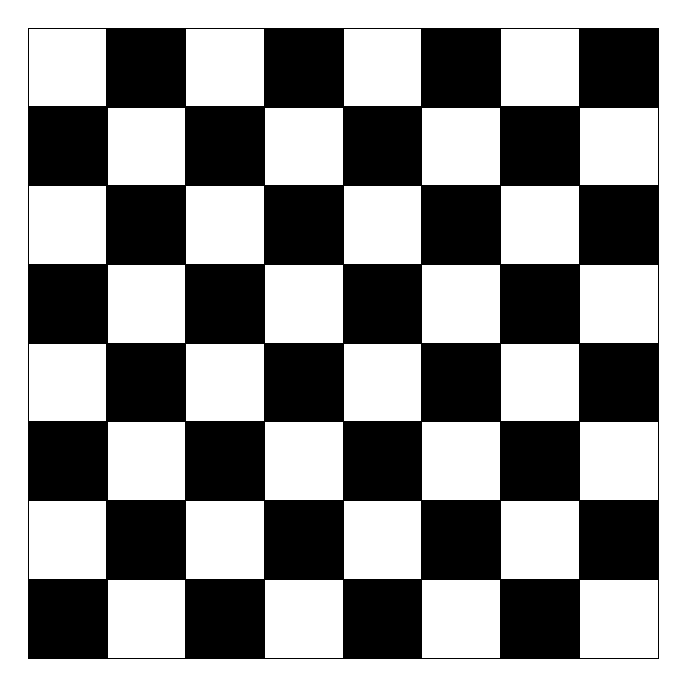
\begin{tikzpicture}
\draw (1,1) rectangle (9,9);
\foreach \x in {1,3,...,8}
\foreach \y in {1,3,...,8}
{ 
\draw[fill=black] (\x,\y) rectangle (\x+1,\y+1);  
\draw[fill=black] (\x+1,\y+1) rectangle (\x+2,\y+2);
}
\end{tikzpicture}
\end{center}

\end{activity}


\end{activities}


\section{Les réferences}

Dans votre document, vous pouvez faire référence aux activités, aux paragraphes du cours ou aux méthodes. En tout cas, celles qui ont été marquées par un \verb!label!.Pour cela, on peut utiliser la commande  \verb!\ref!, mais la commande \verb!\cref! (du package cleveref) donne un meilleur rendu. 

\begin{tcblisting}{colback=red!5!white,colframe=red!75!black,listing above text}
{
\renewcommand{\arraystretch}{2}
\setlength{\tabcolsep}{1cm}
\begin{tabular}{|l|l|}  \hline
\bfseries commande \verb!\ref! &\bfseries  commande \verb!\cref! \\ \hline  
\ref{quart} &
\cref{quart}
\\ \hline 
\ref{partie_exos} &
\cref{partie_exos}
\\ \hline 
\ref{echec_et_maths} &
\cref{echec_et_maths} \\ \hline 
\end{tabular}
}
\end{tcblisting}

